\documentclass[conference]{IEEEtran}
\usepackage{filecontents}
\usepackage[noadjust]{cite}
\usepackage[portuguese]{babel}
\usepackage[utf8]{inputenc}
\usepackage{url}
\usepackage{hyperref}
\usepackage{graphicx}
\usepackage{mathtools}
\usepackage{amsmath}

\hyphenation{op-tical net-works semi-conduc-tor}    

\title{Categorização de Crimes em São Francisco - Solução utilizada para uma Competição do Kaggle}

\author{\IEEEauthorblockN{Vítor de Albuquerque Torreão}
\IEEEauthorblockA{DEINFO - UFRPE\\
	Recife, Pernambuco\\
	\href{mailto:vitor.torreao@ufrpe.br}{\texttt{vitor.torreao@ufrpe.br}}}
\and
\IEEEauthorblockN{Dayanne Cristina de Araujo Barbosa}
\IEEEauthorblockA{DEINFO - UFRPE\\
	Recife, Pernambuco\\
	\href{mailto:dayanne.araujo@ufrpe.br}{\texttt{dayanne.araujo@ufrpe.br}}}
\and
\IEEEauthorblockN{Iury Adones Xavier dos Santos}
\IEEEauthorblockA{DF - UFRPE\\
	Recife, Pernambuco\\
	\href{mailto:iuryadones@gmail.com}{\texttt{iuryadones@gmail.com}}}
}


\markboth{Disciplina de Reconhecimento de Padrões, Dezembro~2015}%
{Shell \MakeLowercase{\textit{et al.}}: Bare Demo of IEEEtran.cls for Journals}

\begin{document}
\maketitle

\begin{abstract}
	A cidade de São Francisco, EUA, já foi famosa por abrigar os criminosos mais 
	notórios do mundo na famosa prisão de Alcatraz. Hoje, a cidade e o condado 
	mantém um website de dados abertos que provê um banco de dados sobre os 
	crimes cometidos nos últimos 12 anos. O website de \textit{data science}, 
	Kaggle, lançou uma competição onde cientistas de dados de qualquer lugar do 
	mundo devem usar algoritmos de aprendizagem de máquina para criar modelos 
	que classifiquem corretamente os crimes cometidos na cidade dentro das 
	diferentes categorias.	Este trabalho relata uma abordagem utilizada para 
	classificar crimes e resolver o desafio proposto pelo Kaglle.
\end{abstract}

\begin{table*}[t]
	\centering
	\caption{Matriz de Correlação}
	\label{corrmatrix}
	\begin{tabular}{|l|c|c|c|c|c|c|}
		\hline
		& \textbf{Data} & \textbf{Dia da Semana} & \textbf{Distrito} & \textbf{Latitude} & \textbf{Longitude} & \textbf{Categoria} \\ \hline
		\textbf{Data} & 1.0000 & 0.0007 & 0.0068 & -0.0039 & -0.0088 & -0.0218 \\ \hline
		\textbf{Dia da Semana} & 0.0007 & 1.0000 & -0.0021 & 0.0034 & 0.0002 & 0.0031 \\ \hline
		\textbf{Distrito} & 0.0068 & -0.0021 & 1.0000 & -0.2680 & 0.0167 & -0.0406 \\ \hline
		\textbf{Latitude} & -0.0039 & 0.0034 & -0.2680 & 1.0000 & 0.5593 & -0.0244 \\ \hline
		\textbf{Longitude} & -0.0088 & 0.0002 & 0.0167 & 0.5593 & 1.0000 & -0.0004 \\ \hline
		\textbf{Categoria} & -0.0218 & 0.0031 & -0.0406 & -0.0244 & -0.0004 & 1.0000 \\ \hline
	\end{tabular}
\end{table*}

\begin{IEEEkeywords}
	Aprendizado de máquina, classificação, criminologia, competição.
\end{IEEEkeywords}

\section{Introdução}
De 1934 a 1963, a cidade de São Francisco, Califórnia, Estados Unidos, ficou 
conhecida por abrigar alguns dos mais notórios criminosos do mundo na prisão de 
Alcatraz \cite{alcatraz}. Hoje em dia, apesar da cidade ser mais conhecida por 
seu cenário tecnológico, com a grande desigualdade social,  não há escassez de 
crimes na cidade.

A prefeitura de São Francisco disponibiliza, no seu portal de transparência 
\cite{sf_open_data}, dados abertos sobre relatórios de crimes cometidos ao longo 
de quase 12 anos na cidade.

O portal de \textit{data science} Kaggle \cite{kaggle}, montou uma competição 
aberta ao público mundial. O objetivo é explorar essa base de dados e, dadas 
informações sobre o local e a hora do crime, classificar os crimes dentro da 
categoria correta. Eles proveem um painel de classificação que mostra os times e 
a sua pontuação. Os autores registraram uma equipe chamada  “UFRPE-RP-2015.2”.

\subsection{Objetivos}

Dessa forma, os objetivos do presente trabalho foram: explorar a base de dados 
de crimes cometidos em São Francisco, à procura de propriedades importantes que 
possam guiar a seleção e implementação de um algoritmo de aprendizado de máquina 
para corretamente classificar os padrões disponíveis.

Depois, implementar uma solução para o problema e submetê-la à plataforma de 
competições do Kaggle.

Finalmente, descrever a metodologia utilizada e os resultados obtidos através do 
presente artigo com o propósito de difundir os conhecimentos obtidos sobre 
aprendizado de máquina.

\section{Trabalhos Relacionados}
Este trabalho trata da classificação de crimes através de dados disponibilizados 
pelo Kaggle \cite{kaggle} para uma competição. Dessa forma, encontramos um post 
\cite{efavdb} de uma equipe participante desta mesma competição falando sobre a 
abordagem utilizada explorando o algoritmo Naive Bayes.

No trabalho \cite{Saeed2015}, técnicas de mineração de dados e inteligência 
artificial são utilizadas para fazer previsão de atributos de crimes. É 
importante lembrar que \cite{Saeed2015} se diferencia do desafio que nosso 
trabalho resolve por uma série de fatores: apenas tratamos a classificação e não 
previsão e, além disso, a base de dados usada no trabalho  \cite{Saeed2015} 
possui aproximadamente 128 atributos. Como resultado o Naive Bayes 
\cite{naivebayes} teve maior precisão do que o uso de árvores de decisão 
\cite{decisiontree}.

O trabalho \cite{Shojaee} tem como objetivo utilizar inteligência artificial 
para classificar, prever e resolver crimes. É importante destacar a análise 
comprativa feita aplicando os algoritmos: Naive Bayes\cite{naivebayes}, KNN 
\cite{knn}, redes neurais \cite{redesneurais}, SVM \cite{svm} e árvores de 
decisão \cite{decisiontree}. Novamente, o Naive bayes teve melhores resultados. 
A base de dados utilizada neste trabalho é parecida com a base do trabalho 
\cite{Saeed2015}.

Em \cite{Mcclendon2015}, para detectar e prever crimes é realizada uma análise 
comparativa de algoritmos de inteligência artificial: regressão linear 
\cite{linearregression}, regressão aditiva \cite{additiveregression} e decisão 
stump \cite{decisionstump} em que a regressão linear possui maior precisão.

A maioria dos trabalhos encontrados foram de abordagens mais genéricas para 
classificação e previsão de crimes utilizando técnicas de aprendizado de 
máquina. 

Outra fonte de informações para fundamentar a solução deste trabalho foi o uso 
do fórum do Kaggle para o desafio de categoriazação de crimes 
\cite{kaggleforum}. No fórum, competidores compartilhavam informações e 
esclareciam dúvidas com o objetivo de solucionar o desafio.

\section{A Competição}
Nesta seção serão descritas a competição do Kaggle e as bases de dados 
fornecidas pelo portal para a competição, além de algumas informações extraídas 
que ajudam o leitor a compreender melhor os conjuntos de dados.

A competição proposta em \cite{kaggleforum}, desafia cientistas de dados do 
mundo inteiro a construir classificadores para categorizar crimes ocorridos na 
cidade de São Francisco, nos Estados Unidos.

O Kaggle \cite{kaggle} disponibiliza duas bases de dados: uma para testes e uma 
para treinamento. Estas bases possuem crimes cometidos na cidade de São 
Francisco entre 1 de janeiro de 2003 e 13 de Maio de 2015. A base de testes deve 
ser utilizada pelo competidor para submeter seus resultados. Para cada instância 
da base de testes, deve ser enviado um valor para cada classe do problema, onde 
cada um destes valores corresponde à probabilidade de a instância pertencer à 
classe. A base de treinamento possui 3 campos a mais: a categoria do crime 
(classe que o modelo deve encontrar), como o crime foi resolvido e uma descrição 
do crime. Nota-se que a presença da classe desejada para cada instância torna 
viável a aplicação de algoritmos para aprendizado supervisionado.

A base de treinamento possui 878.049 instâncias, enquanto que a de teste tem 
884.262. São seis atributos em comum:

\begin{itemize}
	\item \textbf{Data:} A data da ocorrência do crime;
	\item \textbf{Dia da Semana:} O dia da semana no qual o crime ocorreu;
	\item \textbf{Distrito:} O distrito do departamento de polícia;
	\item \textbf{Endereço:} o endereço aproximado de onde ocorreu o crime;
	\item \textbf{Latitude:} A latitude onde o crime aconteceu;
	\item \textbf{Longitude:} A longitude onde o crime foi executado.
\end{itemize}


O atributo \textbf{Data} está descrito no formato timestamp, as informações de 
hora e minuto estão presentes. Assim, \textbf{Data} é um atributo quantitativo 
intervalar. \textbf{Dia da Semana} é uma string em inglês com o nome do dia por 
extenso, por exemplo, “Tuesday”. \textbf{Dia da semana} é, portanto, um atributo 
qualitativo ordinal. O \textbf{Distrito} também é fornecido como string. Alguns 
exemplos de valores são: “Northern”, “Southern” e “Central”. Por isso, 
\textbf{Distrito} é um atributo qualitativo nominal. O \textbf{Endereço} é mais 
um atributo string e qualitativo nominal. \textbf{Latitude} e \textbf{Longitude} 
são ambos atributos quantitativos intervalares.

Ao realizar uma submissão na plataforma do Kaggle, o time terá seu modelo 
qualificado através da métrica \textit{multi-class logarithmic loss} 
\cite{logloss}. Esta métrica é calculada da seguinte forma:

$$ logloss = -\frac{1}{N}\sum_{i=1}^N\sum_{j=1}^My_{ij}\log(p_{ij}) $$

Onde $N$ é o número de instâncias na base de testes; $M$ é o número de classes 
distintas; $log$ é a função logaritmo natural \cite{naturallog}; $y_{ij}$ é $1$ 
se a $i$-ésima instância pertence à classe $j$, e $0$ caso contrário; e $p_{ij}$ 
é a probabilidade calculada pelo classificador de a $i$-ésima instância 
pertencer à classe $j$.

Observando a base de treinamento e aplicando algumas ferramentas estatísticas, 
foi possível observar que os atributos disponíveis possuiam uma correlação 
praticamente inexistente, com exceção de Latitude e Longitude, e Latitude e 
Distrito. Este último pode ser explicado pelo fato de os distritos de polícia, 
em São Francisco, estarem dividindo a cidade em porções horizontais de acordo 
com suas localizações específicas. Por exemplo, um dos departamentos de polícia 
é o \textit{Northern}, que fica mais ao norte da cidade, e por tanto, tem uma 
latitude mais alta. O oposto pode ser dito do \textit{Southern}. O leitor pode 
se referir à Tabela~\ref{corrmatrix} para visualizar a matriz de correlação 
completa.

Por conta dessa baixa correlação entre eles, identifica-se que, provavelmente, 
nenhum atributo é reduntante e todos são importantes para classificar os crimes. 
Além disso, observa-se que não existe uma correlação significativa entre nenhum 
atributo das instâncias e suas classes. De fato, intuitivamente, pode-se 
argumentar que o \textit{onde} e o \textit{quando} não são suficientes para 
categorizar um crime.

Além disso, ao observar as instâncias do conjunto de treinamento foi possível 
identificar que as classes se encontram desbalanceadas para este conjunto, vide 
o histograma presente na Figura~\ref{hist}. Sendo \textit{TREA}, invasão ou 
vandalismo em uma área industrial, a classe menos frequênte com apenas 6 
instâncias e \textit{Larceny}, furto, a mais frequente, com mais de 176 mil 
instâncias.

\section{Processo de Desenvolvimento da Solução}

Através de pesquisa bibliográfica e consultas ao fórum do desafio 
\cite{kaggleforum}, foi possível detectar que participantes do desafio e 
trabalhos semelhantes conseguiam bons resultados utilizando algoritmo Naive 
Bayes \cite{naivebayes}. Além disso, trata-se de uma abordagem interessante já 
que a saída do algoritmo é compatível com a entrada solicitada pelo Kaggle: as 
probabilidades do crime pertencer a cada uma das 39 possíveis categorias de 
crime do desafio.

Uma primeira tentativa de utilização do algoritmo Naive Bayes, implementado  
utilizando a API do Weka \cite{weka}, obteve apenas 7\% de taxa de 
classificação utilizando validação cruzada com 10 \textit{folds}. Diante do 
baixo resultado observado, o passo seguinte foi tentar aplicar engenharia de 
atributos \cite{featureengi}, ou seja, utilizar os conhecimentos sobre o domínio 
do problema para tentar melhorar a qualidade dos atributos do conjunto de dados 
e, consequentemente, melhorar a qualidade dos classificadores.

Partindo desse princípio, o atributo data, que antes estava em timestamp, foi 
tratado, quebrando-o em vários pequenos atributos como: Ano, mês, dia, hora e 
minuto para aumentar a taxa de classificação.

O impacto dessa abordagem foi o aumento da taxa de classificação para 19,3\%. 
No entanto, a matriz de confusão exibida pelo WEKA mostrava que o classificador 
estava classificando as instâncias apenas entre as duas classes mais frequêntes.

Diante dessa situação, a abordagem seguinte foi tentar normalizar os atributos e 
discretizá-los, o que aumentou a taxa de classificação para 24\%. A nova matriz 
de confusão também mostrou uma melhora, pois o classificador passou a 
classificar as instâncias em mais classes.

Para este classificador foi calculado também o \textit{logloss}. O valor 
encontrado foi 2,61, o que colocaria a equipe na 452º posição.

\begin{figure}[t]
	\caption{Histograma das classes presentes no conjunto de treinamento}
	\label{hist}
	\centering
	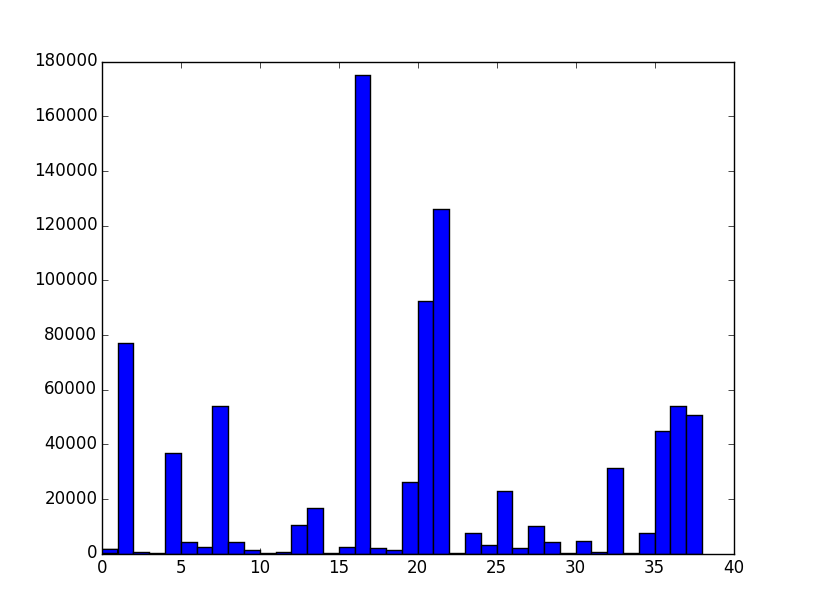
\includegraphics[width=0.45\textwidth]{hist_categoria}
\end{figure}

A próxima tentativa foi a criação de polinômios a partir dos atributos mais 
relevantes para o problema. Assim, foram criados outros seis atributos seguindo 
as seguintes equações:

\begin{equation}
\begin{aligned}
& \text{ano} \times \text{mês} \times \text{dia} \times \text{hora}^2 \\
& \text{hora}^2 \times \text{dia da semana}^3 \times \text{mês} \\
& \text{dia da semana}^3 \times \text{distrito}^2 \\
& \text{latitude} \times \text{longitude} \times \text{distrito}^2 \times \text{rua}^3 \\
& \text{rua}^2 \times \text{dia da semana}^3
\end{aligned}
\end{equation}

Com esses polinômios como novos atributos, foi possível conseguir atingir 26,7\% 
de taxa de classificação com o Naive Bayes do WEKA. E com o \textit{logloss} de 
2,58, a equipe ficaria na 320º posição no \textit{ranking} do Kaggle.

Na tentativa de obter uma nova melhora na classificação, foi utilizada uma 
técnica de engenharia de atributos sugerida por \cite{papadopc}, e proposta em 
\cite{microsoft}, chamada "aprendizado por contagem". Esta técnica se baseaia em 
contar atributos, ou seja, consiste em contar o número de vezes que um valor 
aparece na base de dados e então utilizar esse resultado como um novo atributo 
para treinar o modelo. Este novo atributo pode, então, prover ao modelo uma 
noção da força da evidência deixada por um determinado valor para aquele 
atributo. Dentre os atributos que podem ser criados com a aprendizagem baseada 
em contagem, foi utilizado o \textit{logit}, ou \textit{log odds} \cite{logit}.

Assim, foram criados 39 novos atributos, contendo o \textit{logit} do atributo 
"endereço"\ para cada uma das classes. Além deles, também por sugestão de 
\cite{papadopc}, foram criados novos atributos: um atributo para estação do ano, 
baseado no mês; e um atributo booleano chamado "esquina". Este último atributo é 
verdadeiro se, no campo "endereço", existem os nomes de duas ou mais ruas, e 
falso caso contrário.

Além disso, o atributo "endereço"\ foi transformado de nominal para inteiro 
através de um mapeamento simples e incorporado aos demais atributos.

Devido a sua lentidão no treinamento e alto consumo de memória, a biblioteca do 
WEKA foi abandonada. Sendo substituída pela \textit{SciKit Learn} \cite{sklearn} 
para linguagem de programação Python.

Com essa nova biblioteca e com o conjunto de dados transformados, foram testados 
os algoritmos Naive Bayes e Regressão Logística \cite{logisticreg}.

Com o algoritmo Naive Bayes, foi observado que a taxa de classificação chegou a 
9,1\%. Enquanto que o \textit{logloss} obtido foi de 13,95. Um retrocesso 
comparado com a abordagem anterior. No entanto, utilizando o algoritmo de 
Regressão Logística, a taxa de classificação obtida foi de 30,46\%, e com 
\textit{logloss} de 2.3, o melhor resultado até então.

Dessa forma, o modelo gerado pelo algoritmo de Regresão logística foi utilizado 
para calcular as probabilidades de cada instância do conjunto de testes 
fornecido pelo Kaggle pertencer a cada uma das 39 classes. O resultado disso foi 
submetido como resposta para a plataforma da competição. O resultado foi o 77º 
lugar com \textit{logloss} de 2.37.

\section{Trabalhos Futuros}

Nesta seção serão exploradas algumas alternativas às abordagens apresentadas 
que não puderam ser investigadas por restrições de cronograma do projeto e, 
sendo assim, ficam para futuras iterações.

Alguns algoritmos amplamente utilizados na literatura e que, comumente, obtêm 
bons resultados em outros problemas, precisam ser testados para este problema 
específico de categorização dos crimes em São Francisco. Entre eles, se 
destacam o Multilayer Perceptron \cite{mlp} e os Support Vector Machines 
\cite{svm}. No entanto, esses algoritmos possuem como características o elevado 
tempo de treinamento, especialmente para bases com muitos atributos e, 
principalmente, muitas instâncias como o a da presente pesquisa.

Outras estratégias de transformação para os atributos podem ser investigadas 
na tentativa de melhorar as métricas de performance apresentadas nesta pesquisa. 
Por exemplo, investigar o uso da estratégia de polinômios em conjunto com a 
abordagem da aprendizagem por contagem. Pode-se ainda avaliar a aplicação de 
algoritmos de seleção de atributos após a aplicação da aprendizagem por 
contagem.

\section{Conclusão}
No presente trabalho foi apresentada a uma solução para o problema proposto pelo 
Kaggle em uma de suas competições. O problema envolve a categorização de crimes 
ocorridos na cidade de São Francisco.

Começando por uma análise dos dados disponibilizados pela plataforma, toda a 
estratégia utilizada para se chegar à solução foi descrita com riqueza de 
detalhes.

Além disso, a solução em si obteve bons resultados e figura em boa posição no 
\textit{ranking} do Kaggle. O modelo encontrado é capaz de classificar quase um 
terço das instâncias apresentadas corretamente, além de ter um bom 
\textit{logloss} quando comparado com as melhores soluções. Outra vantagem, 
ainda, é seu baixo tempo para treinamento e execução.

Por fim, foram descritas algumas possíveis formas de incrementar o trabalho e 
melhorá-lo.

\section*{Agradecimentos}
Os autores estendem sua gratidão ao cientista de dados Chris Papadopoulos 
pelos seus inestimáveis \textit{insights} publicados nos fóruns de discussões do 
Kaggle. Os autores são gratos também a Felipe Amorim, professor da Universidade 
Federal Rural de Pernambuco por suas orientações e conselhos ao longo da 
pesquisa.

\bibliography{artigo}
\bibliographystyle{IEEEtran}
\end{document}
